\chapter{Сравнительный анализ моделей}\label{ch3}

В главе \ref{ch3} проводится сравнительный анализ шести моделей, обученных на подготовленных выборках. Цель --- оценить качество предсказания двух ключевых агрономических характеристик: площади покрытия и размера капель. Для обеих задач модели обучались на 80\% данных. Оставшиеся 20\% использовались для тестирования. Результаты сравниваются как по визуальному соответствию предсказаний реальным значениям, так и по метрикам качества --- коэффициенту детерминации $R^2$ (\ref{ch1:R2}) и среднеквадратичной ошибке $RMSE$ (\ref{ch1:RMSE}).

\section{Предсказание площади покрытия}\label{ch3:coverage}

На \firef{fig:coverage-lr} видно, что линейная регрессия не способна точно аппроксимировать зависимости между признаками и покрытием. Предсказания на тестовой выборке значительно отклоняются от истинных значений. Это подтверждается метриками: $R^2 = 0.8616$ и $RMSE \approx 1.03$. Полученные результаты указывают на несоответствие простой линейной модели характеру зависимости в данных, что ожидаемо при высокой размерности пространства признаков.

\begin{figure}[htbp!]
	\centering
	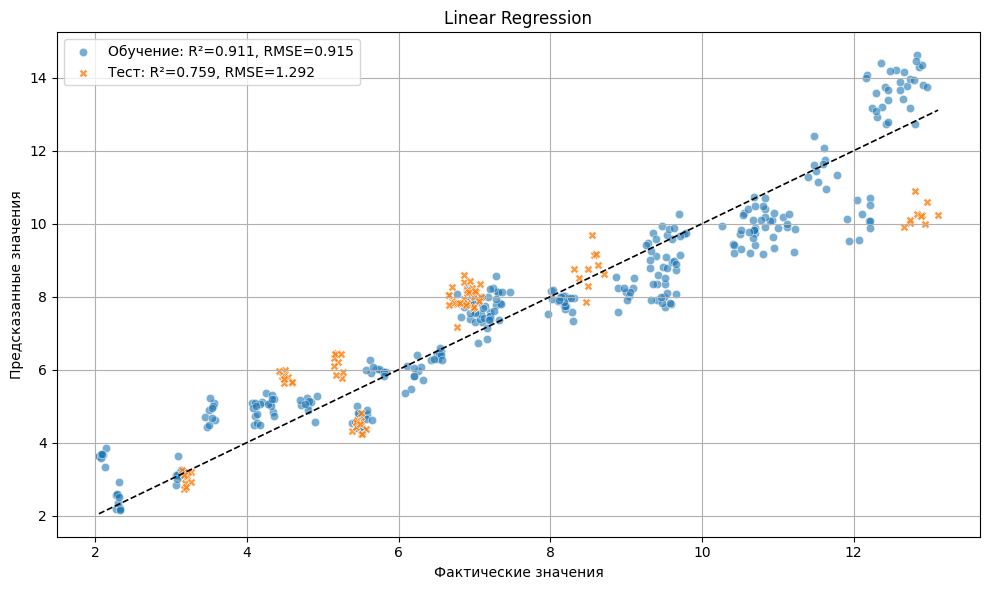
\includegraphics[width=.9\linewidth]{my_folder/images/coverage/Linear-Regression.png}
	\caption{Предсказания линейной регрессии (LR)} 
	\label{fig:coverage-lr}  
\end{figure}

SVR, использованный с подобранными параметрами методом поиска на сетке с оценкой через кросс-валидацию, показывает значительно более точные предсказания (\firef{fig:coverage-svr}). Хотя на тестовой выборке наблюдается небольшое расхождение, модель в целом хорошо справляется с задачей. Повышенная гибкость SVR позволила уловить часть нелинейных зависимостей, обеспечив $R^2 = 0.9308$ при умеренной $RMSE \approx 0.73$.

\begin{figure}[htbp!]
	\centering
	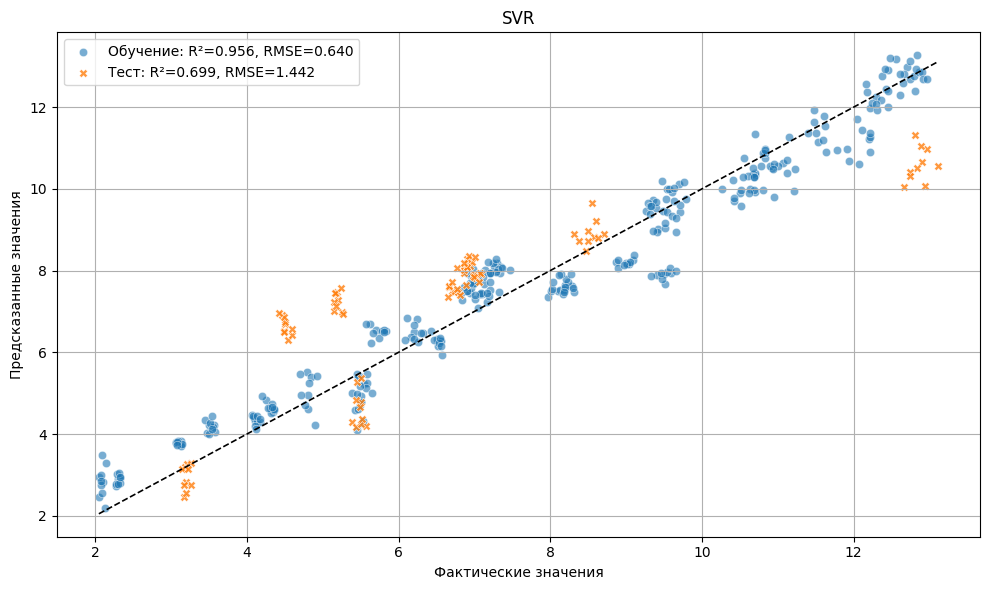
\includegraphics[width=.9\linewidth]{my_folder/images/coverage/SVR.png}
	\caption{Предсказания метода опорных векторов (SVR)} 
	\label{fig:coverage-svr}  
\end{figure}

Случайный лес продемонстрировал устойчивые и сбалансированные результаты (\firef{fig:coverage-rf}). Несмотря на некоторую тенденцию к переобучению ($R^2 = 0.9950$ на обучении), на тестовой выборке модель сохраняет высокую точность --- $R^2 = 0.9521$, $RMSE \approx 0.61$. Предсказания визуально соответствуют истинным значениям.

\begin{figure}[htbp!]
	\centering
	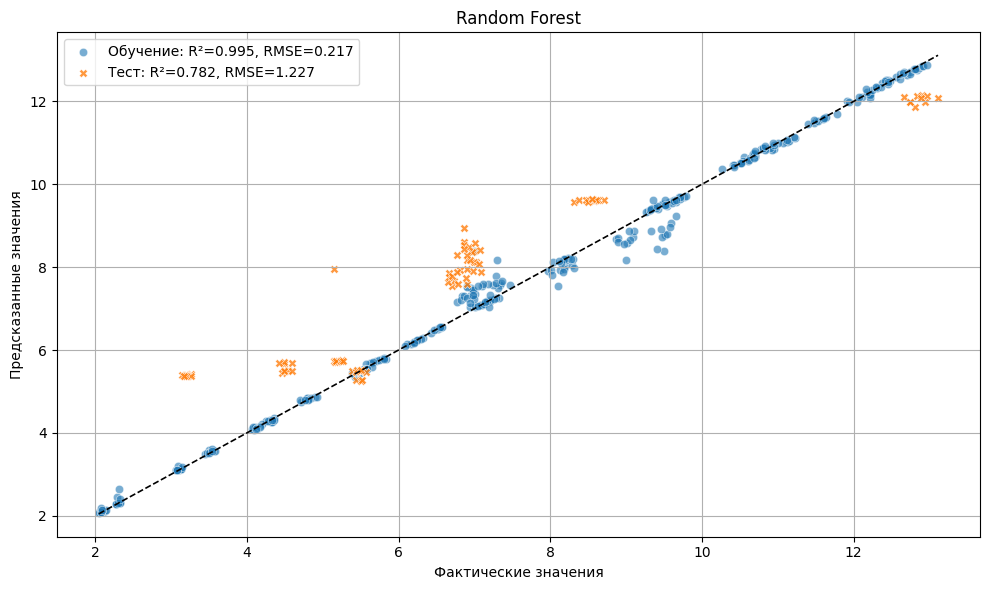
\includegraphics[width=.9\linewidth]{my_folder/images/coverage/Random-Forest.png}
	\caption{Предсказания метода случайного леса (RF)} 
	\label{fig:coverage-rf}  
\end{figure}

Модель градиентного бустинга (\firef{fig:coverage-gbr}) показывает схожие с RF результаты. Наблюдается незначительное ухудшение предсказаний на тестовой выборке по сравнению с обучающей ($R^2 = 0.9472$, $RMSE \approx 0.64$), однако разброс предсказаний невелик.

\begin{figure}[htbp!]
	\centering
	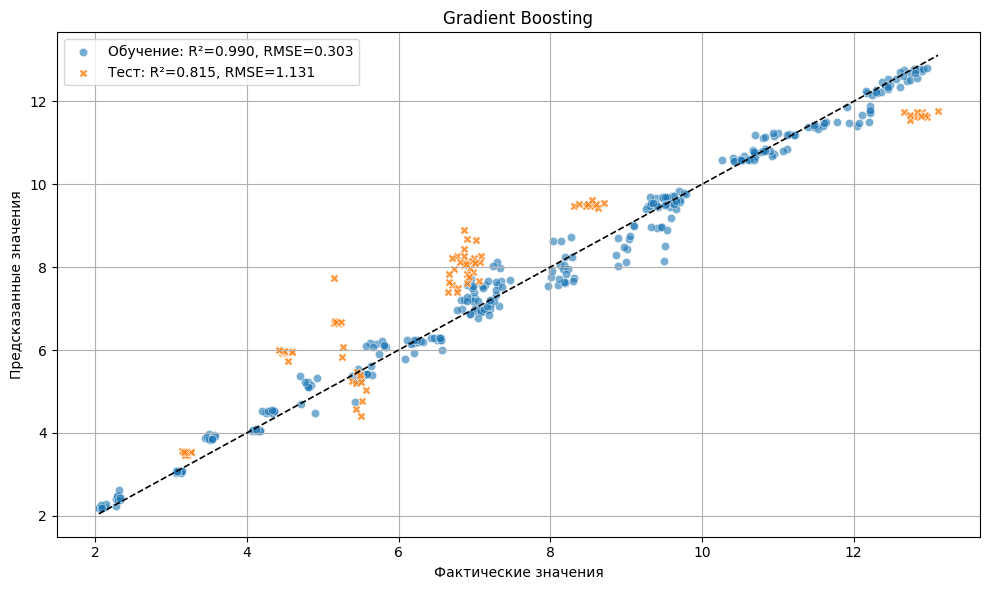
\includegraphics[width=.9\linewidth]{my_folder/images/coverage/Gradient-Boosting.png}
	\caption{Предсказания метода случайного леса (RF)} 
	\label{fig:coverage-gbr}  
\end{figure}

На \firef{fig:coverage-xgboost-overfit}  отражён эффект явного переобучения XGBoost при использовании параметров по умолчанию. Модель почти идеально аппроксимирует обучающую выборку ($R^2 = 0.9994$, $RMSE = 0.085$), однако тестовая точность резко снижается ($R^2 = 0.9028$, $RMSE \approx 0.86$), что свидетельствует о слабой способности к обобщению. 

\begin{figure}[htbp!]
	\centering
	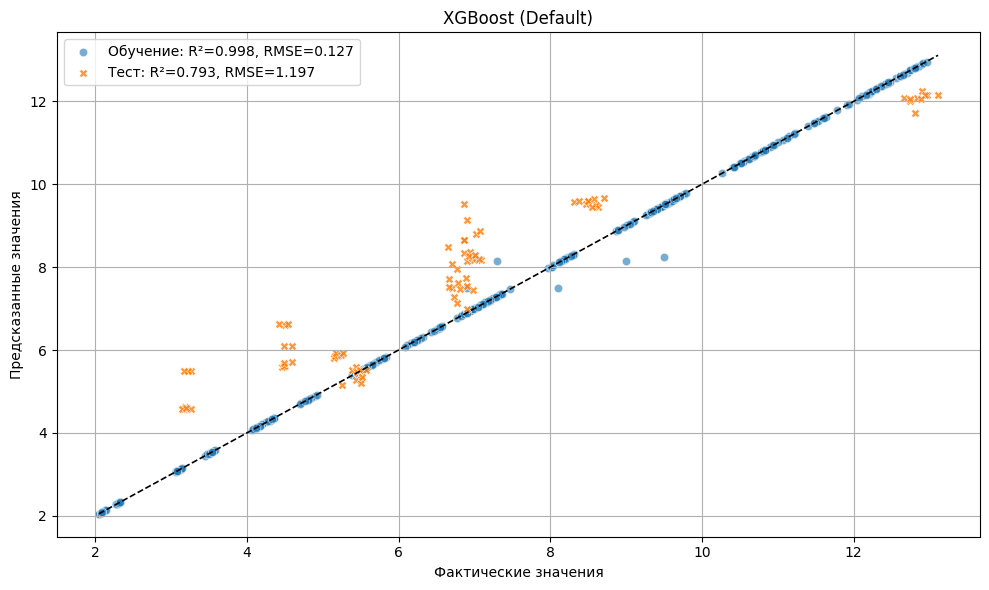
\includegraphics[width=.9\linewidth]{my_folder/images/coverage/XGBoost-overfiting.png}
	\caption{Предсказания XGBoost до настройки параметров} 
	\label{fig:coverage-xgboost-overfit}  
\end{figure}

После настройки с помощью генетического алгоритма модель XGBoost продемонстрировала заметное улучшение (\firef{fig:coverage-xgboost}). Хотя она всё ещё уступает CatBoost и RF, разница между обучающей и тестовой метриками снижается.

\begin{figure}[htbp!]
	\centering
	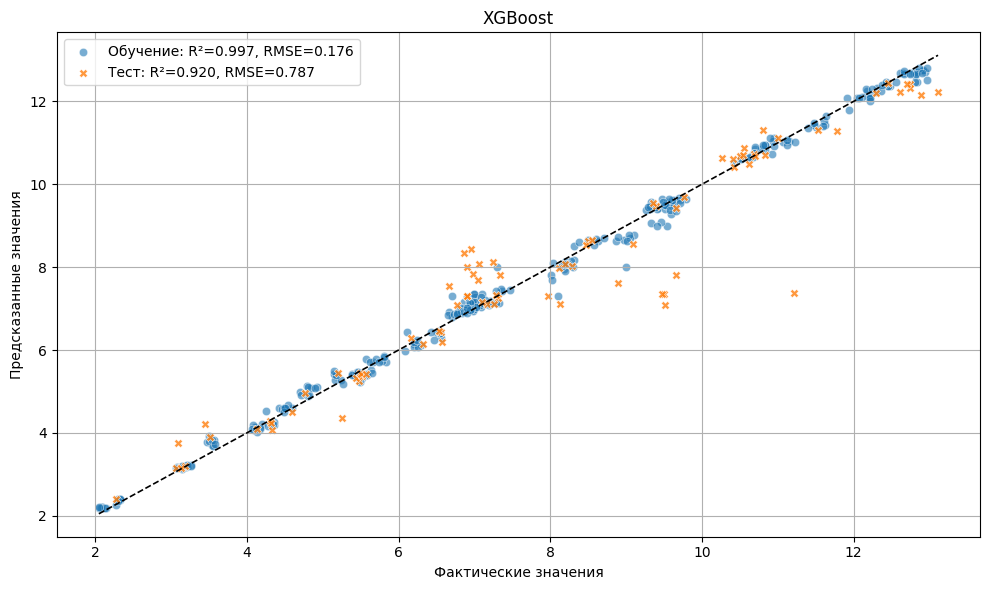
\includegraphics[width=.9\linewidth]{my_folder/images/coverage/XGBoost.png}
	\caption{Предсказания XGBoost после настройки параметров} 
	\label{fig:coverage-xgboost}  
\end{figure}


CatBoost оказался наиболее устойчивым алгоритмом среди всех рассмотренных. Как показано на \firef{fig:coverage-catboost}, предсказания на тестовой выборке плотно группируются вдоль диагонали и почти не отличаются от обучающей выборки. Метрики ($R^2 = 0.9789$, $RMSE \approx 0.40$) подтверждают превосходство CatBoost в задаче предсказания площади покрытия.

\begin{figure}[htbp!]
	\centering
	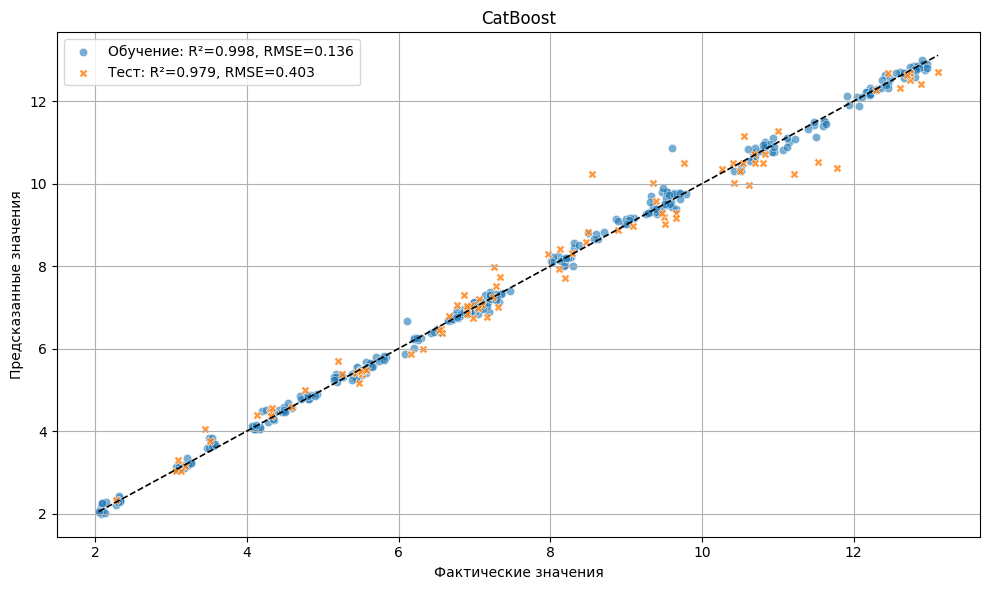
\includegraphics[width=.9\linewidth]{my_folder/images/coverage/CatBoost.png}
	\caption{Предсказания модели CatBoost} 
	\label{fig:coverage-catboost}  
\end{figure}

В \taref{tab:coverage-table} отражены значения метрик для каждой модели:

\begin{table}[htbp!]
	\centering\small
	\caption{Сводная таблица $R^2$ и $RMSE$ для площади покрытия}
	\label{tab:coverage-table}		
	\begin{tabular}{|l|c|c|c|c|}
		\hline
		\multirow{2}{*}{Модель} & \multicolumn{2}{|c|}{Обучающая выборка} & \multicolumn{2}{c|}{Тестовая выборка}\\\cline{2-5} 
		& $R^2$ & $RMSE$ & $R^2$ & $RMSE$\\\hline
		CatBoost&0.998025&0.135801&0.978861&0.403143\\
		RandomForest&0.995028&0.215485&0.952139&0.606611\\
		GradientBoosting&0.988823&0.323084&0.946735&0.639943\\
		SVR&0.968489&0.542478&0.930807&0.729373\\
		XGBoost&0.996682&0.176043&0.919520&0.786617\\
		LinearRegression&0.903087&0.951350&0.861556&1.031707\\
		\hline
	\end{tabular}	
	\normalsize
\end{table}

Они подтверждают сделанные ранее предположения: CatBoost достиг наилучшего баланса между обучением и обобщением. Следом идут RF и GBR с незначительным отставанием. SVR занял промежуточную позицию, а XGBoost, несмотря на мощность, требует тонкой настройки. Линейная регрессия, ожидаемо, замыкает список по точности.

\section{Предсказание диаметра капель}\label{ch3:droplet-size}

Как и в задаче покрытия, линейная регрессия не смогла качественно справиться с прогнозированием размера капель. На \firef{fig:droplet-size-lr} видно сильное отклонение предсказаний от действительных значений. Метрики подтверждают низкую точность модели ($R = 0.8531$, $RMSE \approx 22.52$).

\begin{figure}[htbp!]
	\centering
	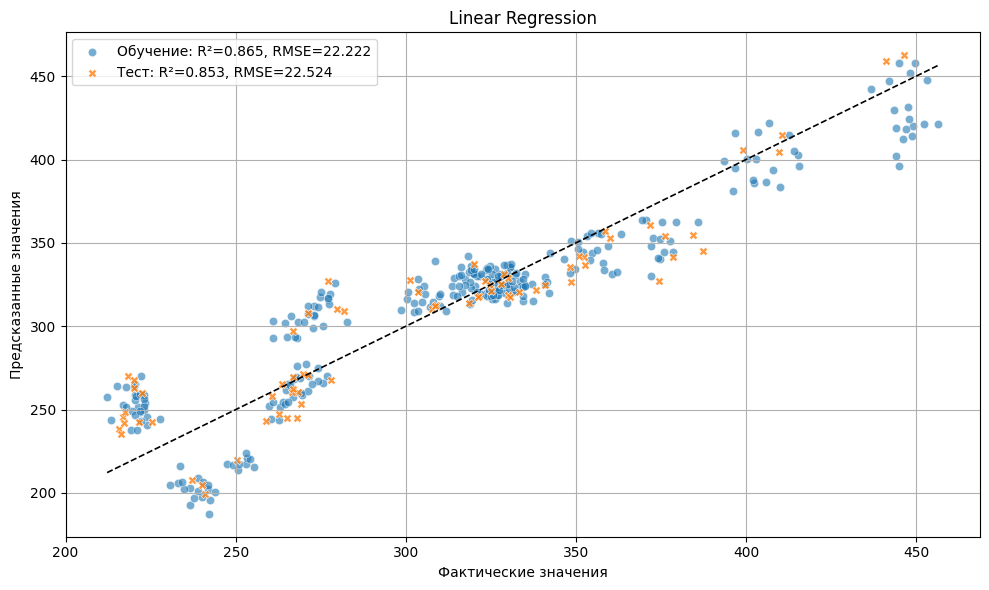
\includegraphics[width=.9\linewidth]{my_folder/images/droplet_size/Linear-Regression.png}
	\caption{Предсказания линейной регрессии (LR)} 
	\label{fig:droplet-size-lr}  
\end{figure}

SVR показала наилучший результат. На \firef{fig:droplet-size-svr} почти все точки располагаются вдоль диагонали. При $R^2 = 0.9869$ и $RMSE \approx 6.72$ модель показывает как высокую точность, так и стабильность на тестовой выборке.

\begin{figure}[htbp!]
	\centering
	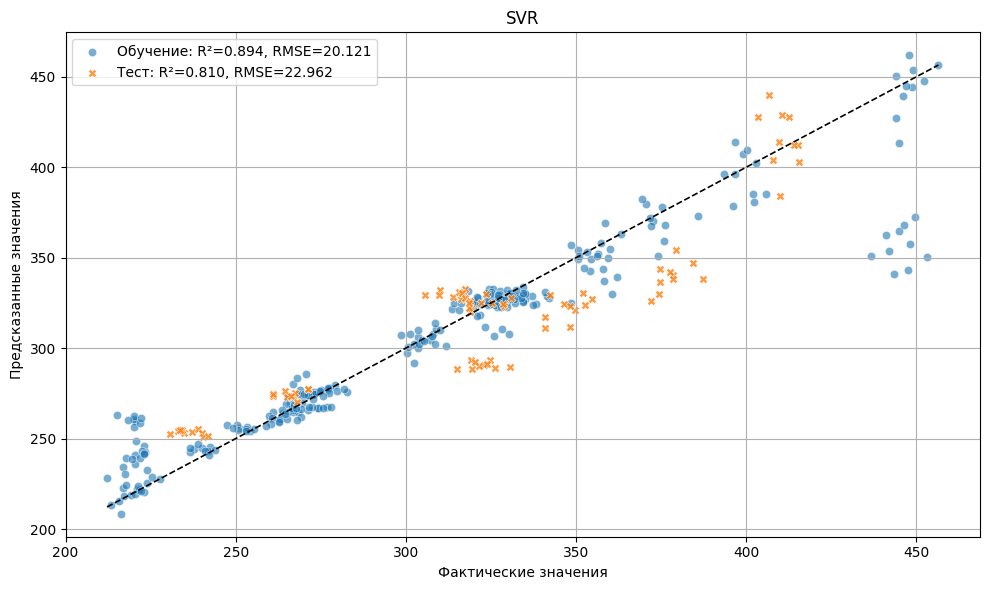
\includegraphics[width=.9\linewidth]{my_folder/images/droplet_size/SVR.png}
	\caption{Предсказания метода опорных векторов (SVR)} 
	\label{fig:droplet-size-svr}  
\end{figure}

Случайный лес (\firef{fig:droplet-size-rf}) также отражает высокую точность, особенно при обучении, но на тесте точность ниже по сравнению с SVR ($R^2 = 0.9770$, $RMSE \approx 8.91$).

\begin{figure}[htbp!]
	\centering
	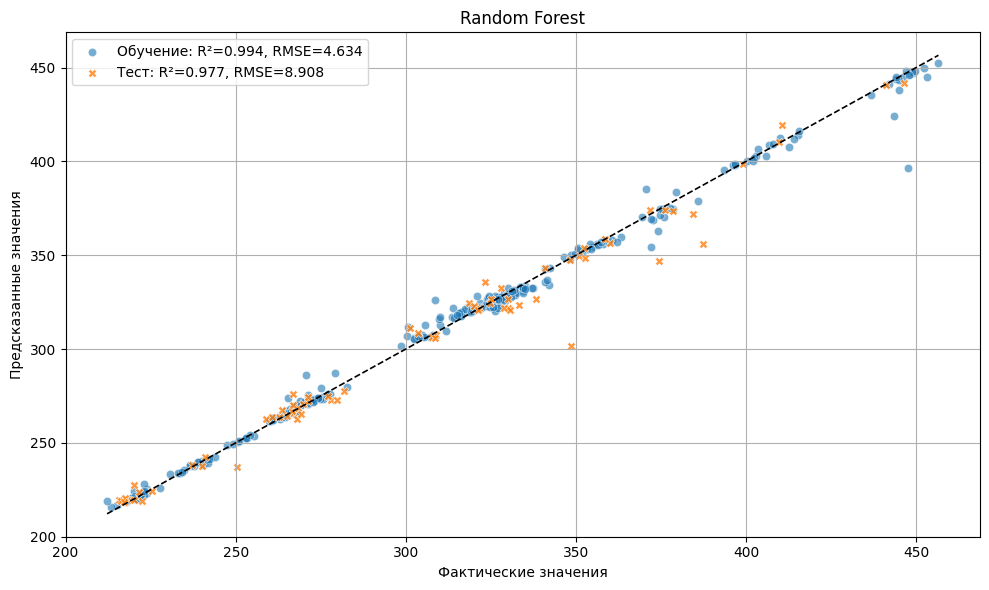
\includegraphics[width=.9\linewidth]{my_folder/images/droplet_size/Random-Forest.png}
	\caption{Предсказания метода случайного леса (RF)} 
	\label{fig:droplet-size-rf}  
\end{figure}

Несмотря на наибольший $RMSE \approx 15.43$ среди ансамблевых моделей, Gradient Boosting (\firef{fig:droplet-size-gbr}) показал приемлемое качество на тестовой выборке ($R^2 = 0.9311$). График предсказаний указывает, что высокая ошибка объясняется единичным выбросом, тогда как основная масса точек лежит близко к идеальной диагонали.

\begin{figure}[htbp!]
	\centering
	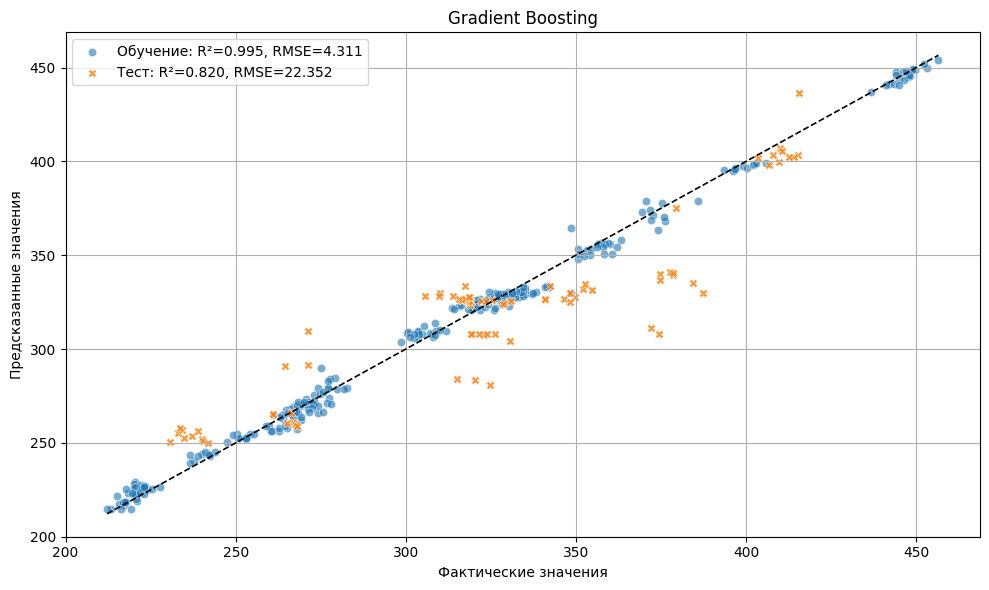
\includegraphics[width=.9\linewidth]{my_folder/images/droplet_size/Gradient-Boosting.png}
	\caption{Предсказания метода случайного леса (RF)} 
	\label{fig:droplet-size-gbr}  
\end{figure}

Для задачи предсказания диаметра капель XGBoost также подвержен переобучению. На \firef{fig:droplet-size-xgboost-overfit} видно почти полное совпадение предсказаний на обучении ($R^2 = 0.9999$, $RMSE \approx 0.62$), но значительное снижение точности на тесте ($R^2 = 0.9228$, $RMSE \approx 16.30$). Несмотря на настройку (\firef{fig:droplet-size-xgboost}), модель остаётся чувствительной к неравномерному распределению данных в выборке, что отражается в снижении качества предсказаний ($R^2 = 0.9707$, $RMSE \approx 10.05$).

\begin{figure}[htbp!]
	\centering
	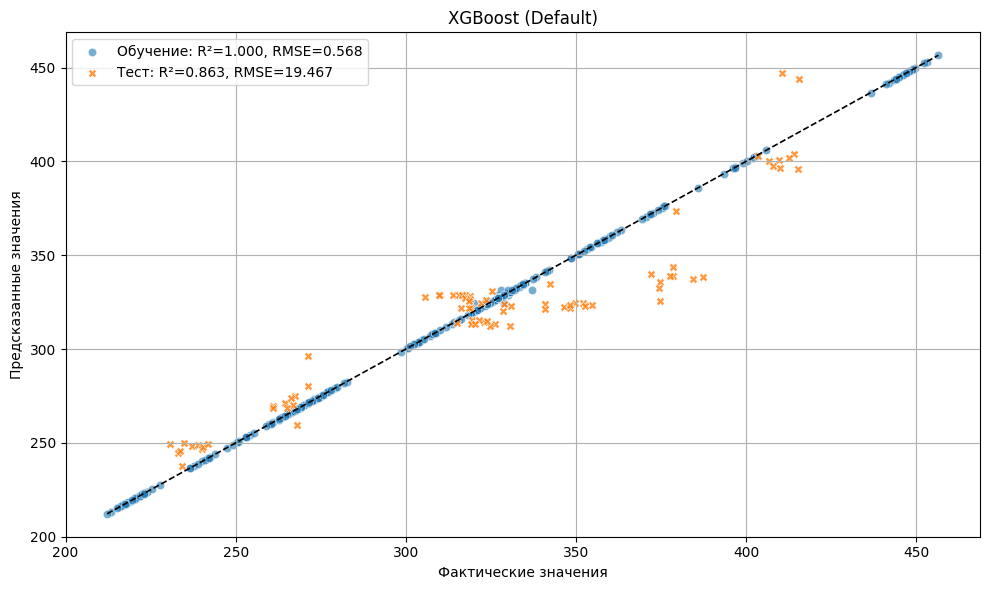
\includegraphics[width=.9\linewidth]{my_folder/images/droplet_size/XGBoost-overfiting.png}
	\caption{Предсказания XGBoost до настройки параметров} 
	\label{fig:droplet-size-xgboost-overfit}  
\end{figure}

\begin{figure}[htbp!]
	\centering
	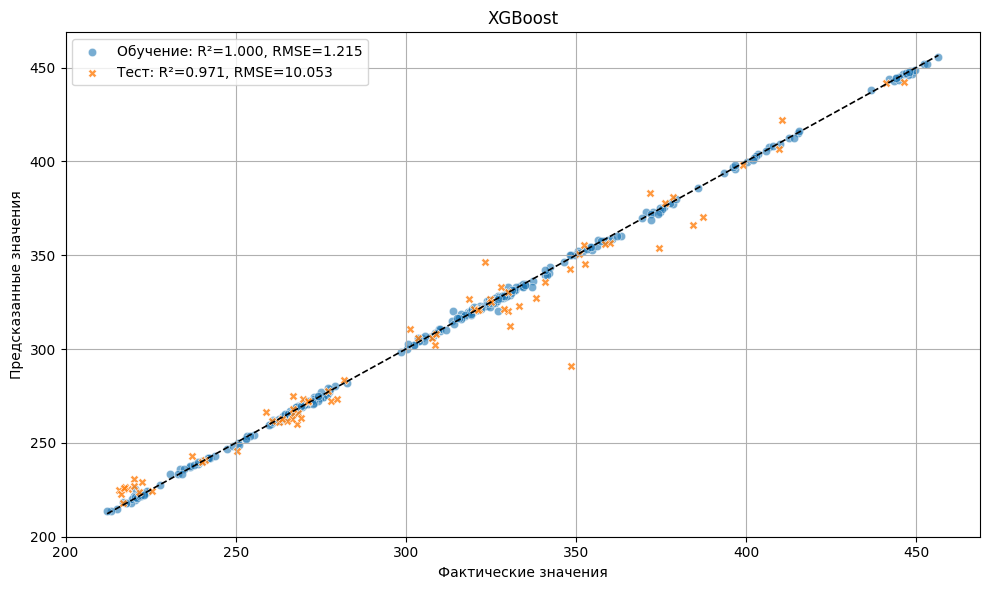
\includegraphics[width=.9\linewidth]{my_folder/images/droplet_size/XGBoost.png}
	\caption{Предсказания XGBoost после настройки параметров} 
	\label{fig:droplet-size-xgboost}  
\end{figure}

\newpage

CatBoost вновь продемонстрировал высокую стабильность и точность. Хотя он немного уступил SVR и RF на тесте ($R^2 = 0.9746$, $RMSE \approx 9.37$), его общее поведение --- надёжное и предсказуемое. На \firef{fig:droplet-size-catboost} предсказания плотно прилегают к диагонали.

\begin{figure}[htbp!]
	\centering
	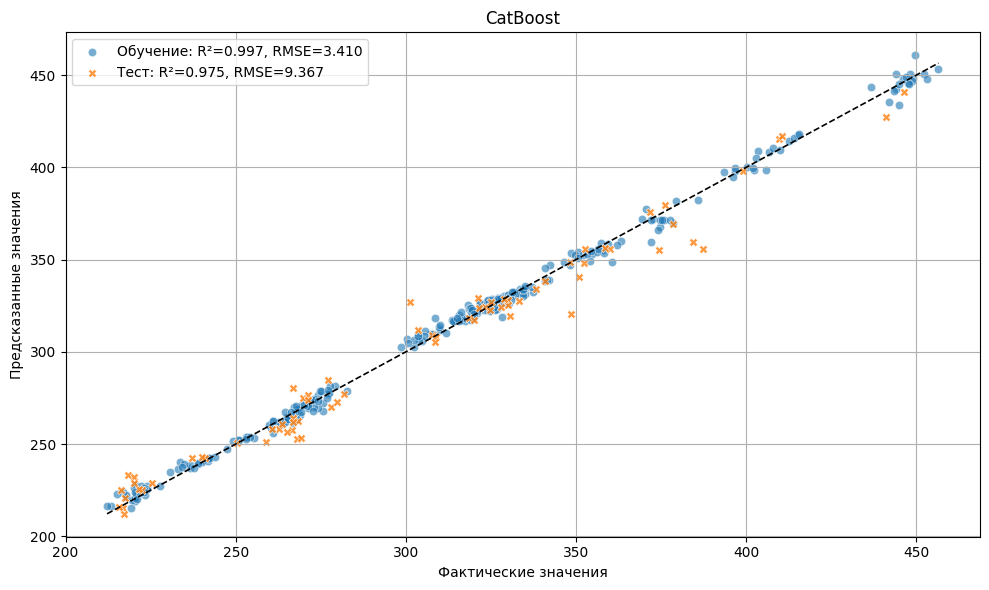
\includegraphics[width=.9\linewidth]{my_folder/images/droplet_size/CatBoost.png}
	\caption{Предсказания модели CatBoost} 
	\label{fig:droplet-size-catboost}  
\end{figure}

В \taref{tab:droplet-size-table} сведены все значения метрик, полученные при предсказании диаметров капель:

\begin{table}[htbp!]
	\centering\small
	\caption{Сводная таблица $R^2$ и $RMSE$ для диаметра капель}
	\label{tab:droplet-size-table}		
	\begin{tabular}{|l|c|c|c|c|}
		\hline
		\multirow{2}{*}{Модель} & \multicolumn{2}{|c|}{Обучающая выборка} & \multicolumn{2}{c|}{Тестовая выборка}\\\cline{2-5} 
		& $R^2$ & $RMSE$ & $R^2$ & $RMSE$\\\hline
		SVR&0.989895&6.081541&0.986923&6.719734\\
		RandomForest&0.994133&4.633962&0.977019&8.907997\\
		CatBoost&0.996822&3.410447&0.974588&9.367232\\
		XGBoost&0.999596&1.215277&0.970734&10.052552\\
		GradientBoosting&0.991920&5.438013&0.931059&15.428785\\
		LinearRegression&0.865076&22.222023&0.853068&22.524294\\
		\hline
	\end{tabular}	
	\normalsize
\end{table}

Значения подтверждают, что наилучшие результаты обеспечили SVR и CatBoost. XGBoost, несмотря на хорошие показатели на обучении, уступил по обобщающей способности. Random Forest и Gradient Boosting показали хорошие, но менее стабильные результаты: оба алгоритма склонны к ухудшению качества при переходе от обучающей выборки к тестовой. Линейная регрессия снова показала худшие результаты, особенно по $RMSE$.

\section{Выводы}

По итогам анализа можно заключить, что CatBoost является наиболее универсальной и надёжной моделью, демонстрируя высокую точность и устойчивость как в задаче предсказания покрытия, так и диаметра капель. SVR, при правильной настройке гиперпараметров, обеспечивает высокую точность в задаче предсказания диаметра, но несколько уступает в задаче покрытия. XGBoost требует обязательной оптимизации, чтобы избежать переобучения. Случайный лес (RF) и градиентный бустинг (GBR) демонстрируют хорошие результаты с параметрами по умолчанию, но уступают CatBoost по стабильности. Линейная регрессия (LR) также показала наихудшие результаты и, соответственно, не пригодна для описания сложных зависимостей в рассматриваемых агрономических задачах.

